\chapter{Groundwork}
Before implementing the system, some groundwork was done regarding the available data:

\section{Wifi Signal Strength study}

The behaviour of the wifi signal strength distribution for a stationary laptop 
and smartphone was analyzed to characterize the input wifi signal.

\subsection{Short term duration}

Figure \ref{fig:closestAPshortterm} shows the variation of signal strength of 
the closest AP for a smartphone placed within a room in a NON-LOS configuration.

\begin{figure}\centering
    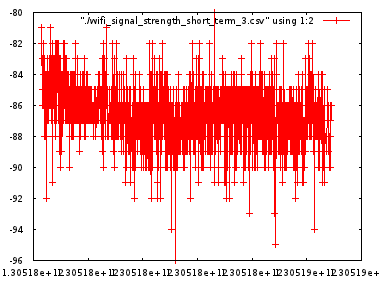
\includegraphics{figures/short_term_wifi.png}
    \caption{Variation of RSSI for closest AP. \label{fig:closestAPshortterm}}
\end{figure}


\subsection{During a thunderstorm}

Figure \ref{fig:closestAPthunderstorm} shows the variation of signal strength of
the closest AP for a smartphone placed in a room in NON-LOS configuration.

\begin{figure}\centering
    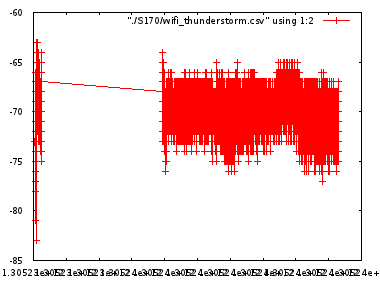
\includegraphics{figures/wifi_thunderstorm.png}
    \caption{Variation of RSSI for closest AP during a thunderstorm. \label{fig:closestAPthunderstorm}}
\end{figure}

\subsection{7 day study}

The Wifi AP RSSI values were monitored over a 7 day period (Jan 5 2011 - Jan 13 2011) from room S-152
and the resulting signal strength data was analyzed.

\begin{figure}\centering
    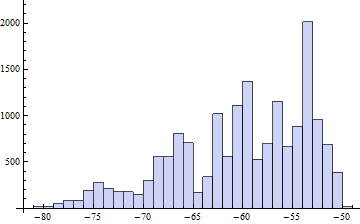
\includegraphics{figures/histogram_00_1C_F0_CB_EC_92.png}
    \caption{Distribution of RSSI values for the closest AP (00:1C:F0:CB:EC:92) \label{fig:histogram_00_1C_F0_CB_EC_92}}
\end{figure}

As you can see in Figure \ref{fig:histogram_00_1C_F0_CB_EC_92}, the signal strength
distribution is highly non-gaussian. This kind of distribution makes Kalman filters
unsuitable for use as the assumptions of gaussian (linear) distribution of 
input variables is unsatisfied.

\begin{figure}\centering
    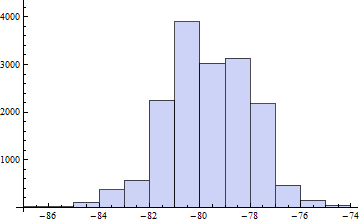
\includegraphics{figures/histogram_00_1C_F0_CB_EC_95.png}
    \caption{Distribution of RSSI values for the AP near S-170 (00:1C:F0:CB:EC:95) \label{fig:histogram_00_1C_F0_CB_EC_95}}
\end{figure}

\begin{figure}\centering
    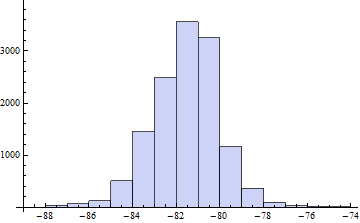
\includegraphics{figures/histogram_00_19_5B_77_A5_EE.png}
    \caption{Distribution of RSSI values for the AP near S-159 (00:19:5B:77:A5:EE) \label{fig:histogram_00_19_5B_77_A5_EE}}
\end{figure}

\begin{figure}\centering
    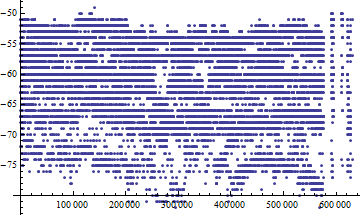
\includegraphics{figures/listplot_00_1C_F0_CB_EC_92.png}
    \caption{Point plot of RSSI values for the closest AP (00:1C:F0:CB:EC:92) \label{fig:listplot_00_1C_F0_CB_EC_92}}    
\end{figure}

\begin{figure}\centering
    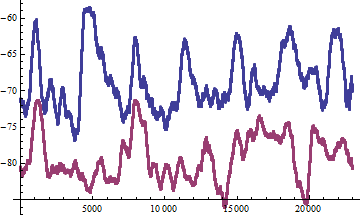
\includegraphics{figures/moving_average.png}
    \caption{3 hour moving average of RSSI values}
\end{figure}

Figure \ref{fig:histogram_00_19_5B_77_A5_EE} doesn't show such a pronounced non-gaussian
nature whereas Figure \ref{fig:histogram_00_1C_F0_CB_EC_95} shows more leanings towards a
non-gaussian distribution.

Figure \ref{fig:listplot_00_1C_F0_CB_EC_92} is the time domain plot of the signal strength
samples. As you can see, the samples can be spread over a large domain even if the 
sample times differ by a couple of hours. Thus we can safely conclude that the 
input wifi signal is a highly noisy source of information.

\section{Effect of motion on signal strengths}

To analyze the effect of motion on the RSSI values from the APs, a simple walking
test was done along a corridoor. The variation of RSSI values seen from the APs in
the corridoor are shown in \ref{fig:wifi_corridoor_walk}.

\begin{figure}\centering
    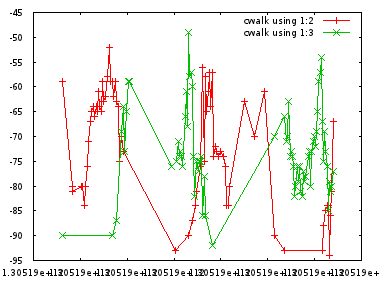
\includegraphics{figures/wifi_corridoor_walk.png}
    \caption{RSSI values for APs during a corridoor walk \label{fig:wifi_corridoor_walk}}
\end{figure}

TODO: Improve figure with more APs and path description.

\subsection{Inferences}
Effect of orientation with respect to AP is important. Signal strength values
even in LOS situations don't always behave nicely.

\section{Wifi Surveying}

A $1m x 1m$ grid was set up on the ground and wifi readings were taken at 8
different orientations per point on the floor.

\clearpage
\section{Implementation of a KNN based positioning solution for KNN accuracy}

A KNN based location system was implemented to test location accuracy. 
This was work done as part of the project. Results are included here.

\begin{table}[h]
    \centering
    \caption{Performance of KNN based indoor positioning system \label{tab:knnperf}}
    \begin{tabular}{|l|c|c|c|}
    \hline
              & Mean Error $\bar{e}$ (m) & $\sigma_{error}$ (m) & $\bar{e} + 2 \sigma_{error}$ \\
    \hline
    \hline
    $K = 1$    & 2.8 & 2.7 & 8.2 \\
    $K = 2$    & 2.8 & 2.7 & 8.2 \\
    $K = 3$    & 2.7 & 2.7 & 8.1 \\
    $K = 4$    & 2.3 & 2.8 & 7.9 \\
    \hline
    \end{tabular}

\end{table}


\subsection{Improvements}
Use of SVM is likely to improve the accuracy further at room level. [Redpin]

\section{Magnetometer}

The Nexus S comes with a built in [insert smartphone chip info] MEMS magnetometer.
It measures the local magnetic field strength in $\mu T$.

\subsection{Accuracy}
The performance is reasonable but the magnetometer has a lot of sensor noise and suffers from
sensor bias. For example, rotation of the smartphone through large angles introduces bias
in the readings from the magnetometer.

\begin{figure}\centering
    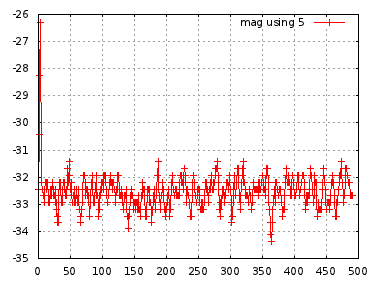
\includegraphics{figures/mag_z_table.png}
    \caption{Magnetometer readings when device is on a table \label{fig:mag_z_table}}
\end{figure}

\begin{figure}\centering
    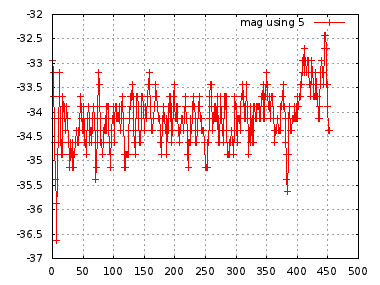
\includegraphics{figures/mag_z_handheld_standing.png}
    \caption{Magnetometer readings when device is held in user's hand\label{fig:mag_z_handheld_standing}}
\end{figure}

\begin{figure}\centering
    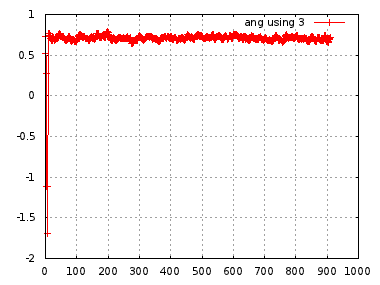
\includegraphics{figures/angle_stationary_table.png}
    \caption{Derived azimuth angle when smartphone on table}
\end{figure}

\begin{figure}\centering
    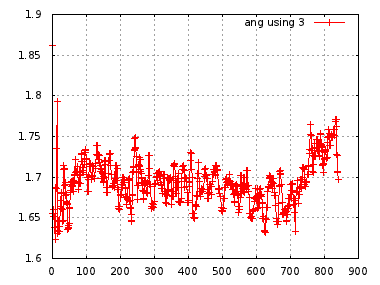
\includegraphics{figures/angle_handheld_standing.png}
    \caption{Derived azimuth angle when smartphone held in hand}
\end{figure}


TODO: Insert values for Standard deviation here.

These values are required to determine choice of parameters for the particle
filter that will be introduced later.

\subsection{Bias study}

Performing rotations in a slow and steady manner yields good results with little
or no bias and sensor lag. See figure \ref{fig:angle_180_rotation_table} which 
shows how the angle measurements behave when the rotated slowly and steadily.

There is only a slight sensor lag and bias visible. However, at steady state,
there is sensor noise of approximately 5 degrees present.

\begin{figure}\centering
    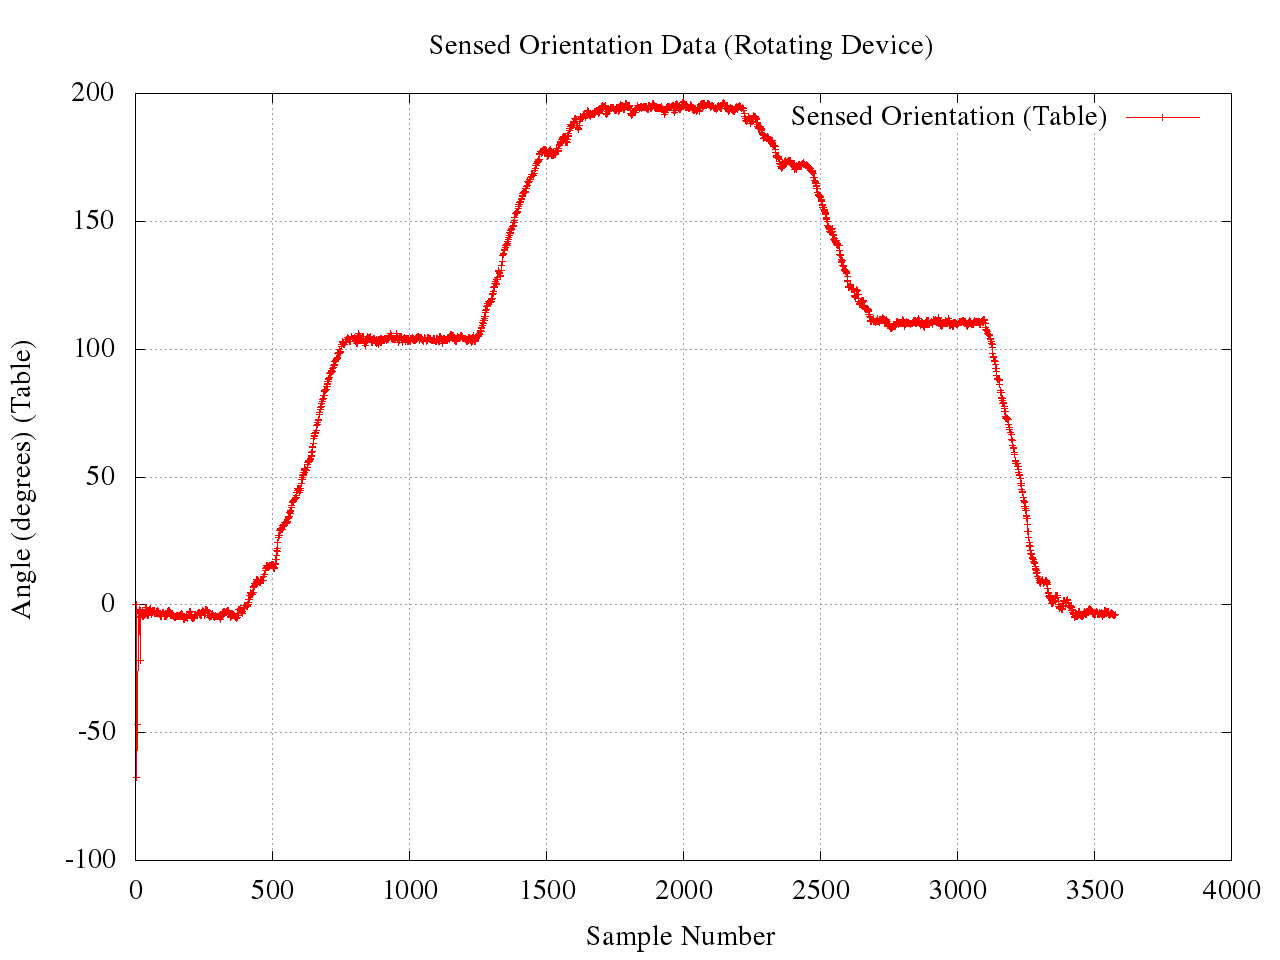
\includegraphics{figures/angle_180_rotation_table.png}
    \caption{Rotation of the phone through 180 degrees with pauses at 90 degrees.\label{fig:angle_180_rotation_table}}
\end{figure}


\subsection{Effect of motion}

Although the sensor measurements are stable when the device is on a table,
the measurements go haywire when the device is in a human's hand. See figure
\ref{fig:angle_180_corridoor} - a human is walking along a corridoor and he walks
back. The angle measurements of the return trip are offset by 180 degrees and
the two sets of measurements are compared. You can easily see a large variation
in the angles due to the motion of the human and the dynamic nature of the environment.
Sensor lag and long term sensor value drift is evident in the graph.
This dynamic variation of the measurement of the angle from magnetic north 
introduces error in the inertial navigation system.

\begin{figure}\centering
    \includegraphics{figures/angle_180_corridoor.png}
    \caption{Angle measurements when moving in opp directions.\label{fig:angle_180_corridoor}}
\end{figure}


\section{Accelerometer Study}

The MEMS accelerometer on the Nexus S was also subject to similar characterization.
See figure \ref{fig:accel_static}.

\begin{figure}\centering
    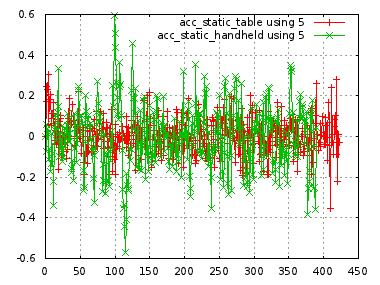
\includegraphics{figures/accel_static.png}
    \caption{Accelerometer Z axis readings when device stationary\label{fig:accel_static}}
\end{figure}


\clearpage
\section{What Doesn’t work}
Acceleration of the human body is too slow compared to gravity. Simple orientation changes produce high changes in acceleration along axes which are very difficult to filter out.
Numerical integration generates errors too quickly. With a high sampling rate, errors balloon.
Using the gyroscope for step detection (similar to foot mounted devices [insert reference]) – doesn’t work.

\section{Other issues}
Sensor noise, instability and bias. Effect of gravity and orientation on readings. Weather.

